\chapter{YÖNETİŞİM, RİSK YÖNETİMİ VE UYUMLULUK (GRC)}

\section*{Giriş}

Bu bölüm, bir kuruluşun siber güvenlik duruşunun temel yapıtaşlarını oluşturan, stratejik ve operasyonel GRC (Yönetişim, Risk ve Uyum) mekanizmalarını derinlemesine incelemektedir. Odak noktası, yalnızca teknik kontrollere odaklanmak yerine, güvenliği bir iş önceliği haline getiren ve kuruluşun hedefleriyle hizalayan entegre bir yaklaşım sunmaktır. GRC, organizasyonun güvenli ve doğru yolda kalmasını sağlayan strateji ve yapı olarak işlev görür, bir tripod gibi yönetim, risk yönetimi ve uyumluluk ayaklarını birleştirir.

\section{Uyum Yönetimi ve Düzenleyici Çerçeveler}

\section{Bilgi Güvenliği Yönetişim Çerçevesi}

Bilgi güvenliği yönetişimi, liderlik, organizasyonel yapılar ve süreçlerden oluşan, bilgi varlıklarını korumayı amaçlayan yapılandırılmış bir çerçevedir. Bu çerçeve, güvenliğin "nedenini", "ne olduğunu" ve "kimin sorumlu olduğunu" ele alarak, taktiksel güvenlik tedbirlerinin ötesine geçer ve stratejik bir iş fonksiyonu olarak konumlanmasını sağlar. Bu, yalnızca teknoloji odaklı bir yaklaşımdan ziyade, organizasyonel hedefler ve risk toleransı ile uyumlu güvenlik uygulamalarını garanti eder.

\subsection{Board-level Security Governance ve Oversight (Yönetim Kurulu Seviyesi Siber Güvenlik Gözetimi)}

Yönetim kurulu seviyesinde siber güvenlik gözetimi, siber risklerin kurumsal risk yönetimi (ERM) stratejisinin ayrılmaz bir parçası olarak kabul edilmesini sağlar. Yönetim kurulunun rolü, detaylı teknik operasyonlara müdahale etmekten ziyade, stratejik yönü belirlemek ve kaynakların etkin bir şekilde ayrılmasını sağlamaktır.

Bu katmanda güvenlik, teknik bir konudan stratejik bir iş konusuna dönüşür. Bir siber olayın yol açabileceği itibar kaybı, finansal cezalar ve iş sürekliliği kesintileri gibi doğrudan iş sonuçları, bu risklerin yalnızca teknik değil, aynı zamanda finansal ve operasyonel riskler olarak algılanmasını zorunlu kılar. Bu geniş etki alanı, yönetim kurulunun bütçe onayı, strateji belirleme ve genel gözetim kapsamında bu konuyu aktif olarak ele almasını gerektirir. Bu dönüşüm, güvenlik liderlerinin (örneğin CISO), teknik jargon yerine iş diliyle (risk, yatırım getirisi (ROI), iş etkisi gibi) konuşma becerisine sahip olmasının önemini ortaya koymaktadır. Yönetim kurulu desteği, kaynak tahsisi ve politika onayı için hayati öneme sahiptir.

Yönetim kurulu düzeyinde etkili gözetim mekanizmalarının temel taşları şunlardır:
\begin{itemize}
    \item \textbf{Siber Okuryazarlığın Artırılması:} Yönetim kurulu üyelerinin, genel siber riskler ve şirketi etkileyen özel siber riskler hakkında bilgi edinmesi esastır. Bu, özel eğitimler ve uzmanlarla yapılan görüşmelerle sağlanabilir.
    \item \textbf{Düzenli Raporlama:} Yönetim kurulu, siber güvenlikten sorumlu yöneticilerle düzenli olarak görüşmeli ve şirketin siber olgunluğunu ve dayanıklılığını anlamalarını sağlayan uygun metrikleri talep etmelidir. Bu metrikler, kolayca toplanabilen verilerden ziyade, en riskli alanlara odaklanmalıdır.
    \item \textbf{Görevlerin Ayrılması:} Siber güvenlik stratejisinin belirlenmesi ve bu stratejinin uygulanması arasında görev ayrımının sağlanması kritik öneme sahiptir. Bu, hesap verebilirliği ve etkinliği artırır.
\end{itemize}

\subsection{Information Security Strategy ve Policy Development (Bilgi Güvenliği Stratejisi ve Politika Geliştirme)}

Kapsamlı bir bilgi güvenliği stratejisi ve politikası, sürekli gelişen tehditlere ve karmaşık uyumluluk gereksinimlerine karşı koordineli ve uygulanabilir bir program oluşturur. Bu strateji, organizasyonun tüm güvenlik süreçlerini uçtan uca kapsayan, uygulanabilir ve iş hedeflerine odaklanmış olmalıdır.

Politika geliştirme süreci, tek seferlik bir olaydan ziyade döngüsel bir yapıya sahiptir. Süreç, risk değerlendirmesiyle başlar, ancak politikanın kendisi de risk yönetimi süreçlerinin etkinliğini ölçmek için kullanılır. Bu yaklaşım, güvenlik duruşunun dinamik ve sürekli değişen bir ortamda güncel kalmasını garanti eder.

Bir bilgi güvenliği politikasının adım adım geliştirilmesi için şu adımlar izlenmelidir:
\begin{enumerate}
    \item \textbf{Mevcut Durum ve Risk Değerlendirmesi:} Sürecin ilk adımı, kuruluşun mevcut güvenlik durumunu, hassas verilerini (PII, finansal belgeler vb.), sistemlerini ve potansiyel zayıflıklarını belirleyen kapsamlı bir risk değerlendirmesi yapmaktır. Bu aşama, aynı zamanda organizasyon için kabul edilebilir risk seviyelerini de tanımlar.
    \item \textbf{Yasal ve Sektörel Gereksinimlerin Belirlenmesi:} İlgili tüm yerel, ulusal ve sektörel yasa ve standartlar (KVKK, GDPR, HIPAA, ISO 27001 vb.) incelenir. Bu, politikanın yasal yükümlülüklerle uyumlu olmasını sağlar.
    \item \textbf{Strateji ve Politika Geliştirme:} Değerlendirme sonuçlarına dayanarak, iş hedefleriyle uyumlu bir bilgi güvenliği stratejisi oluşturulur. Bu stratejinin temelini oluşturan yüksek seviyeli ilkeler, ardından detaylı ve konu bazlı politikalara (örneğin, kabul edilebilir kullanım, erişim kontrolü, parola politikası, şifreleme politikası) dönüştürülür. Politika, gizlilik, bütünlük ve erişilebilirlik gibi temel güvenlik hedeflerine odaklanmalıdır.
    \item \textbf{Onay ve İletişim:} Geliştirilen politikalar üst yönetimden onay almalı ve tüm paydaşlara şeffaf bir şekilde iletilmelidir. Politikanın etkinliğini ölçmek için düzenli olarak risk değerlendirmeleri yapılmalı ve bu değerlendirmeler sonucunda belirlenen iyileştirme alanlarına göre politika güncellenmelidir.
\end{enumerate}

\subsection{Security Organization Structure ve Roles/Responsibilities (Güvenlik Organizasyon Yapısı ve Görev/Sorumluluklar)}

Etkili bir yönetişim için net bir organizasyon yapısı ve tanımlanmış roller hayati öneme sahiptir. Siber güvenlik yönetişimi, görev ve sorumlulukların katmanlı bir yapıda olduğunu gösterir.
\begin{itemize}
    \item \textbf{Yönetim Kurulu:} En üst düzeyde stratejik gözetim sağlar ve siber güvenliğin iş hedefleriyle uyumunu denetler. Bu, en üst düzeyde sorumluluk ve hesap verebilirliği tesis eder.
    \item \textbf{Bilgi Güvenliği Komitesi:} Stratejik düzeyde karar alıcı organdır. Kaynak ayrılması, kabul edilebilir risk seviyelerinin belirlenmesi ve risk işleme aksiyonlarının onaylanması gibi görevleri üstlenir. Bu katman, stratejiyi somut eylemlere dönüştüren bağlayıcı noktadır.
    \item \textbf{Bilgi Güvenliği Koordinasyon Ekibi:} Stratejik hedeflerin operasyonel olarak uygulanmasından sorumludur. Risk değerlendirmesi, varlık envanteri oluşturma ve acil durumlarda hasar tespiti gibi çalışmaları yürütür.
    \item \textbf{Bilgi Güvenliği Yöneticisi / Siber Güvenlikten Sorumlu Yetkili Yönetici (SGSYY):} Yönetim sistemi içindeki rol ve sorumlulukları denetler, güvenlik sorunlarına müdahale eder ve gerekli koordinasyonu sağlar.
\end{itemize}

Bu katmanlı yapı, her seviyede şeffaflık ve hesap verebilirlik sağlayarak, güvenliğin tek bir kişiye veya departmana yüklenmesini engeller. Bu, GRC'nin üçayağının (Yönetişim-Risk-Uyum) işlevsel olarak birleştirilmesini de destekler.

\subsection{Security Culture Development ve Awareness Programs (Güvenlik Kültürü Geliştirme ve Farkındalık Programları)}

Güvenlik kültürü, çalışanların güvenliği önceliklendirdiği ve ortak bir sorumluluk olarak gördüğü bir ortamdır. Zira birçok güvenlik ihlali, oltalama saldırıları veya kullanıcı hatalarından kaynaklanır.

Güvenlik kültürü oluşturmak, sadece eğitimlerle sınırlı kalmamalı, sürekli ve katılımcı bir süreç olmalıdır. Bu süreç, üst yönetimin desteğiyle başlar; yönetim kademesi, güvenlik standartlarını belirleyerek ve güvenliği teşvik ederek örnek olmalıdır. Ardından, çalışanlara düzenli olarak siber güvenlik eğitimleri verilmelidir. Bu eğitimler, kimlik avı saldırılarını tespit etme, parola yönetimi, fiziksel güvenlik ve çıkarılabilir medya kullanımı gibi konuları içermelidir.

Pratik uygulamalar ve simülasyonlar, teorik bilgilerin pekiştirilmesi için kritik öneme sahiptir. Oltalama (phishing) simülasyonları gibi pratik testler, çalışanların riskli davranışlarını değerlendirmek ve güvenli alışkanlıklar geliştirmelerine yardımcı olmak için kullanılmalıdır.

\textbf{Adım Adım Oltalama (Phishing) Simülasyonu Yürütme Kılavuzu:}
\begin{enumerate}
    \item \textbf{Hedef Kitleyi Belirleyin:} Simülasyonun hangi çalışan gruplarını veya departmanlarını hedefleyeceğini netleştirin.
    \item \textbf{Senaryo Oluşturun:} Mevcut şablonlardan veya sıfırdan bir senaryo seçin. Senaryolar genellikle gerçek dünyadaki oltalama tekniklerini taklit eder. Popüler senaryo örnekleri şunlardır:
    \begin{itemize}
        \item \textbf{CEO Dolandırıcılığı:} Üst düzey bir yöneticinin acil para transferi talep ettiği bir e-posta, duygusal ve hiyerarşik bir tetikleyici kullanır.
        \item \textbf{Sahte Şifre Sıfırlama:} LinkedIn gibi güvenilir bir platformdan geldiği iddia edilen, acil şifre sıfırlama uyarısı içeren bir e-posta, aciliyet hissi yaratır.
        \item \textbf{İnsan Kaynakları Politikası Güncellemesi:} Çalışanlara iç ve rutin görünen, yeni bir sağlık hizmeti planı veya ödeme politikası hakkında bilgi veren bir e-posta.
    \end{itemize}
    \item \textbf{Simülasyonu Yapılandırın:} Oltalama e-postasının içeriğini ve yönlendireceği sahte web sayfasını hazırlayın. Bu aşamada, sahte bir giriş sayfası veya zararlı bir dosya indirme bağlantısı içeren bir "yük" (payload) yapılandırılır.
    \item \textbf{Kampanyayı Başlatın:} Simülasyonu başlatma ve bitiş tarihlerini belirleyin. Hedef kitleye otomatik olarak e-postalar gönderilecektir.
    \item \textbf{Sonuçları İzleyin ve Raporlayın:} Kampanya sonuçları (tıklama oranları, veri girişi, raporlama sayısı) izlenerek, riskli kullanıcılar ve güvenlik açıkları belirlenir.
    \item \textbf{Eğitim Ataması:} Başarısız olan çalışanlara otomatik olarak düzeltici eğitimler atanır. Bu, sadece bir test değil, aynı zamanda sürekli bir öğrenme sürecidir.
\end{enumerate}

\subsection{Third-party Risk Governance ve Vendor Management (Üçüncü Taraf Risk Yönetimi ve Tedarikçi Yönetimi)}

Üçüncü taraflara (tedarikçiler, iş ortakları, bulut servis sağlayıcıları) olan bağımlılık arttıkça, bu tarafların yarattığı riskleri yönetmek hayati hale gelmektedir. Kaynaklar, tek bir tedarikçiye aşırı bağımlılığın (single-source) maliyeti optimize edebilse de, operasyonel zafiyetler yarattığını ve iş sürekliliğini tehdit ettiğini belirtmektedir. Uzun süreli ve başarılı vendor ilişkileri, risklerin ortadan kalktığına dair yanlış bir güven duygusu yaratabilir. Bu durum, izleme ve acil durum planlaması çabalarını azaltmaya yol açabilir. Coğrafi olarak aynı bölgede bulunan birden fazla tedarikçi de, doğal afetler gibi lokal olayların tedarik zincirini aynı anda kesintiye uğratmasına neden olabilir.

Bu riskleri yönetmek için kapsamlı bir Üçüncü Taraf Risk Yönetimi (TPRM) programı kurulmalıdır:
\begin{enumerate}
    \item \textbf{Kapsam ve Envanter:} Tedarik zinciri haritasını çıkararak tüm tedarikçileri, hizmet sağlayıcıları ve yüklenicileri kapsamlı bir şekilde listelemekle başlanır.
    \item \textbf{Riske Dayalı Değerlendirme:} Tüm üçüncü taraflara aynı risk değerlendirme süreci uygulanmamalıdır. Bunun yerine, riske orantılı bir yaklaşım benimsenerek, hassas verilere erişenler gibi kritik tedarikçilere daha derinlemesine incelemeler yapılmalıdır.
    \item \textbf{Durum Tespiti (Due Diligence):} Yeni bir tedarikçi ile çalışmaya başlamadan önce, siber güvenlik duruşu, finansal istikrar ve uyumluluk geçmişi gibi konularda kapsamlı bir durum tespiti yapılmalıdır. Bu, kabul edilemez risk seviyelerine sahip tedarikçilerle çalışmaktan kaçınmayı sağlar.
    \item \textbf{Sözleşmeler ve SLA'lar:} Tedarikçilerle imzalanan sözleşmeler ve hizmet seviyesi anlaşmaları (SLA), beklentileri açıkça belirlemeli ve olası kesintilere karşı bir koruma sağlamalıdır.
    \item \textbf{Sürekli İzleme ve Denetim:} Tedarikçi risk profillerindeki değişiklikler düzenli olarak değerlendirilmeli ve gerektiğinde denetimler yapılmalıdır. Bu, risklerin dinamik doğasına uyum sağlamak için esastır.
\end{enumerate}

\section{Kurumsal Risk Yönetimi ve Siber Risk}

Risk yönetimi, işletmenin hedeflerine ulaşmasını engelleyebilecek olumsuz sonuçlara yol açabilecek her şeyi yönetme sürecidir. Bu süreç, belirsizliği ortadan kaldırmayı ve uyumluluk gerekliliklerini karşılamayı amaçlar.

\subsection{ISO 31000 Risk Management Framework (ISO 31000 Risk Yönetim Çerçevesi)}

\textbf{NIST Risk Yönetim Çerçevesi (RMF)}, altı aşamalı bir risk yaşam döngüsü sunar: Kategorize Et, Seç, Uygula, Değerlendir, Yetkilendir ve İzle. Bu sistematik yaklaşım, organizasyonların siber güvenlik risklerini kapsamlı bir şekilde yönetmesini sağlar.

ISO 31000:2018, bir yönetim sistemi standardı olmamasına rağmen, organizasyonların riskleri tanımlaması, analiz etmesi ve yönetmesi için sistematik bir rehber sunar. Bu çerçeve, kuruluşların risk bilincini artırarak karar alma süreçlerini destekler ve sürdürülebilir başarıyı teşvik eder.

Standardın temel ilkeleri şunları içerir:
\begin{itemize}
    \item \textbf{Entegre Yaklaşım:} Risk yönetimi, tüm iş süreçlerine ve karar alma mekanizmalarına entegre edilmelidir.
    \item \textbf{Özelleştirilmiş ve Esnek Olmak:} Çerçeve, her organizasyonun kendine özgü ihtiyaçlarına göre uyarlanabilmelidir.
    \item \textbf{İnsan ve Kültür Faktörleri:} İnsanların algıları ve kültürel faktörler risk yönetiminin başarısını doğrudan etkiler.
    \item \textbf{Sürekli İyileştirme:} Risk yönetimi dinamik bir süreçtir ve sürekli öğrenme ile geliştirilmelidir.
\end{itemize}

\subsection{FAIR (Factor Analysis of Information Risk) Risk Analiz Metodolojisi}

FAIR, bilgi riskini nicel olarak ölçmek için tasarlanmış sistematik bir metodoloji ve uluslararası standart (ISO/IEC 27005 eki) olarak kabul edilmiştir. Geleneksel risk değerlendirmelerinde sıkça karşılaşılan "yüksek-orta-düşük" gibi subjektif değerlendirmelerin yerine, finansal etkiyi sayısal olarak hesaplayabilen bir yaklaşım sunar.

\textbf{FAIR Temel Modeli:}

FAIR, riski iki ana bileşen olarak tanımlar:
\begin{enumerate}
    \item \textbf{Kayıp Olayı Frekansı (Loss Event Frequency - LEF):} Belirli bir tehdidin belirli bir sürede ne sıklıkla gerçekleşebileceğini tahmin eder.
    \item \textbf{Kayıp Büyüklüğü (Loss Magnitude - LM):} Bir kayıp olayının gerçekleşmesi durumunda ortaya çıkacak finansal etkinin miktarını hesaplar.
\end{enumerate}

Risk = LEF × LM formülü ile hesaplanır.

\textbf{FAIR Detaylı Risk Faktörleri:}

\begin{longtable}{|p{3cm}|p{4cm}|p{6cm}|}
\caption{FAIR Risk Faktörleri ve Hesaplama Yöntemleri}\\
\hline
\rowcolor{tableheadcolor}
\textbf{Ana Faktör} & \textbf{Alt Faktörler} & \textbf{Açıklama ve Hesaplama} \\
\hline
\endfirsthead
\multicolumn{3}{c}{\small\tablename\ \thetable\ -- devamı} \\
\hline
\rowcolor{tableheadcolor}
\textbf{Ana Faktör} & \textbf{Alt Faktörler} & \textbf{Açıklama ve Hesaplama} \\
\hline
\endhead
\hline
\multicolumn{3}{r}{\small Devamı sonraki sayfada} \\
\endfoot
\hline
\endlastfoot
Tehdit Olayı Frekansı & Tehdit Kapasitesi, Kontrol Gücü & Bir tehdit aktörünün saldırı gerçekleştirme yeteneği ve mevcut kontrollerin etkisiz hale getirilme ihtimali \\
\hline
Zafiyet & Kontrol Gücü, Tehdit Kapasitesi & Mevcut güvenlik kontrollerinin zayıflıkları ve tehdit aktörünün bunları istismar etme yeteneği \\
\hline
Birincil Kayıp & Veri Kaybı, Sistem Kaybı & Doğrudan maddi kayıplar: veri kurtarma, sistem yenileme, operasyonel kesinti maliyetleri \\
\hline
İkincil Kayıp & İtibar Kaybı, Yasal Cezalar & Dolaylı etkiler: müşteri kaybı, düzenleyici cezalar, hisse değeri düşüşü \\
\hline
\end{longtable}

\textbf{FAIR Uygulama Adımları:}

\begin{enumerate}
    \item \textbf{Kapsam Tanımlama:} Analiz edilecek varlık, tehdit ve senaryo netleştirilir
    \item \textbf{Veri Toplama:} Geçmiş olaylar, endüstri verileri ve uzman görüşleri toplanır
    \item \textbf{Kalibrasyon:} Belirsizlik aralıkları ve olasılık dağılımları belirlenir
    \item \textbf{Monte Carlo Simülasyonu:} Binlerce senaryo çalıştırılarak risk dağılımı hesaplanır
    \item \textbf{Sonuç Analizi:} 95\% güven aralığı ve beklenen yıllık kayıp (ALE) raporlanır
\end{enumerate}

\subsection{Compliance Framework'leri ve Düzenleyici Gereksinimler}

Modern organizasyonlar, faaliyet gösterdikleri sektörlere ve coğrafi konumlara bağlı olarak çoklu düzenleyici gereksinimleri karşılamak zorundadır. Bu compliance landscape'i karmaşık ve sürekli değişen bir yapı arz etmektedir.

\textbf{Temel Compliance Çerçeveleri:}

\begin{longtable}{|p{2.5cm}|p{3cm}|p{4cm}|p{3cm}|}
\caption{Majör Compliance Framework'leri Karşılaştırması}\\
\hline
\rowcolor{tableheadcolor}
\textbf{Framework} & \textbf{Kapsam} & \textbf{Temel Gereksinimler} & \textbf{Hedef Sektör} \\
\hline
\endfirsthead
\multicolumn{4}{c}{\small\tablename\ \thetable\ -- devamı} \\
\hline
\rowcolor{tableheadcolor}
\textbf{Framework} & \textbf{Kapsam} & \textbf{Temel Gereksinimler} & \textbf{Hedef Sektör} \\
\hline
\endhead
\hline
\multicolumn{4}{r}{\small Devamı sonraki sayfada} \\
\endfoot
\hline
\endlastfoot
ISO 27001 & Bilgi güvenliği yönetim sistemi & 114 kontrol, risk yönetimi, sürekli iyileştirme & Tüm sektörler \\
\hline
SOX & Finansal raporlama & IT kontrolleri, veri bütünlüğü, erişim kontrolleri & Halka açık şirketler (ABD) \\
\hline
GDPR & Kişisel veri koruma & Veri minimizasyonu, izin yönetimi, ihlal bildirimi & AB verileri işleyen tüm org. \\
\hline
KVKK & Kişisel veri koruma & Veri işleme kayıtları, DPO atama, etki analizi & Türkiye'deki organizasyonlar \\
\hline
HIPAA & Sağlık verisi koruma & Şifreleme, erişim kontrolü, denetim kayıtları & ABD sağlık sektörü \\
\hline
PCI DSS & Ödeme kartı verisi & Ağ segmentasyonu, şifreleme, penetrasyon testleri & Ödeme işleyen kuruluşlar \\
\hline
NIST CSF & Siber güvenlik çerçevesi & Belirle, koru, tespit et, müdahale et, kurtar & Kritik altyapılar \\
\hline
\end{longtable}

\textbf{Compliance Program Yönetimi:}

Etkili bir compliance programı, sadece düzenleyici gereksinimleri karşılamakla sınırlı kalmamalı, aynı zamanda organizasyonun risk duruşunu güçlendiren stratejik bir avantaj sağlamalıdır.

\begin{enumerate}
    \item \textbf{Gap Analizi ve Başlangıç Değerlendirmesi:} Mevcut kontroller ile gereksinimler arasındaki boşlukların belirlenmesi
    \item \textbf{Compliance Roadmap Geliştirme:} Önceliklendirme, zaman çizelgeleri ve kaynak planlaması
    \item \textbf{Politika ve Prosedür Geliştirme:} Düzenleyici gereksinimleri operasyonel süreçlere çevirme
    \item \textbf{Kontrolların İmplementasyonu:} Teknik ve idari kontrollerin sistematik uygulanması
    \item \textbf{Sürekli İzleme ve Denetim:} Compliance durumunun düzenli değerlendirilmesi
    \item \textbf{Olay Müdahale ve Raporlama:} Düzenleyici bildirimleri ve düzeltici eylemler
\end{enumerate}

\textbf{Automated Compliance Management:}

Modern compliance yönetimi, otomasyon araçları olmadan sürdürülebilir değildir. GRC platformları şu yetenekleri sağlar:

\begin{itemize}
    \item \textbf{Kontrol Mapping:} Çoklu framework'lerdeki benzer kontrollerin eşleştirilmesi
    \item \textbf{Evidence Collection:} Denetim kanıtlarının otomatik toplanması ve arşivlenmesi
    \item \textbf{Risk Assessment Integration:} Compliance durumunun risk skorlaması ile entegrasyonu
    \item \textbf{Dashboard ve Raporlama:} Yönetim için gerçek zamanlı compliance metrikleri
    \item \textbf{Workflow Automation:} Düzeltici eylem planlarının takibi ve eskalasyonu
\end{itemize}
    \item \textbf{İnsan ve Kültür Odaklı Olmak:} İnsan faktörü ve risk bilinci, sürecin kritik bir parçasıdır. Herkesin sürece dahil edilmesi, risklerin daha iyi anlaşılmasını sağlar.
    \item \textbf{Dinamik ve Sürekli Güncellenen Yapı:} Risk yönetimi, sürekli iyileştirilebilir ve proaktif olmalıdır. Organizasyonlar, potansiyel tehditleri önceden belirleyerek beklenmedik durumlarla karşılaşma olasılığını azaltabilir.
\end{itemize}

\subsection{Cyber Risk Quantification ve Business Impact Analysis (Siber Riskin Nicelleştirilmesi ve İş Etki Analizi)}

Siber riskin nicelleştirilmesi, riskleri soyut terimler ("yüksek/orta/düşük") yerine somut finansal değerlerle ifade etmeyi amaçlayan bir yaklaşımdır. Bu, karar alma süreçlerini daha objektif hale getirir ve güvenlik yatırımlarının iş üzerindeki etkisini net bir şekilde gösterir.

\textbf{İş Etki Analizi (BIA) Adım Adım Yönergesi:}
BIA, bir siber olayın kritik iş operasyonları üzerindeki potansiyel etkilerini sistematik olarak değerlendiren bir süreçtir. BIA'nın çıktıları, Felaket Kurtarma Planı (DRP) için gerekli olan Kurtarma Süresi Hedefi (RTO) ve Kurtarma Noktası Hedefi (RPO) gibi hedeflerin belirlenmesinde temel veri kaynağını oluşturur. Bir BIA, kritik iş süreçlerinin ne kadar süre durabileceğini ve ne kadar veri kaybına dayanabileceğini değerlendirerek, teknik ekiplerin Felaket Kurtarma Planı (DRP) için net RTO ve RPO değerleri belirlemesini sağlar.

BIA'nın temel adımları şunlardır:
\begin{enumerate}
    \item \textbf{Kapsamı Tanımlayın:} Hangi iş birimlerinin, süreçlerinin ve sistemlerinin analize dahil edileceğini netleştirin.
    \item \textbf{Kritik İş Fonksiyonlarını Belirleyin:} Kuruluşun temel operasyonlarını ve hizmetlerini listeleyin. Her bir fonksiyon için potansiyel finansal, operasyonel ve itibar kayıplarını belirleyin.
    \item \textbf{Bağımlılıkları Haritalandırın:} Kritik fonksiyonların hangi IT sistemlerine, verilere, personele ve üçüncü taraf hizmetlerine bağımlı olduğunu çıkarın.
    \item \textbf{Etkileri Değerlendirin:} Her bir kesintinin zaman içindeki (örneğin, ilk birkaç saat, ilk 24 saat, ilk hafta) potansiyel etkilerini (gelir kaybı, yasal cezalar, itibar zedelenmesi) finansal olarak ölçün.
\end{enumerate}

\subsection{FAIR (Factor Analysis of Information Risk) Methodology (FAIR Metodolojisi)}

FAIR, siber riskleri parasal terimlerle nicelleştiren ve subjektif ("yüksek/orta/düşük") değerlendirmelerden objektif, veriye dayalı analize geçişi sağlayan uluslararası bir standarttır. Bu model, güvenlik yatırımlarının işe yaradığını göstermek ve bütçe kararlarını desteklemek için stratejik bir dilde iletişim kurmaya olanak tanır.

\begin{figure}[H]
    \centering
    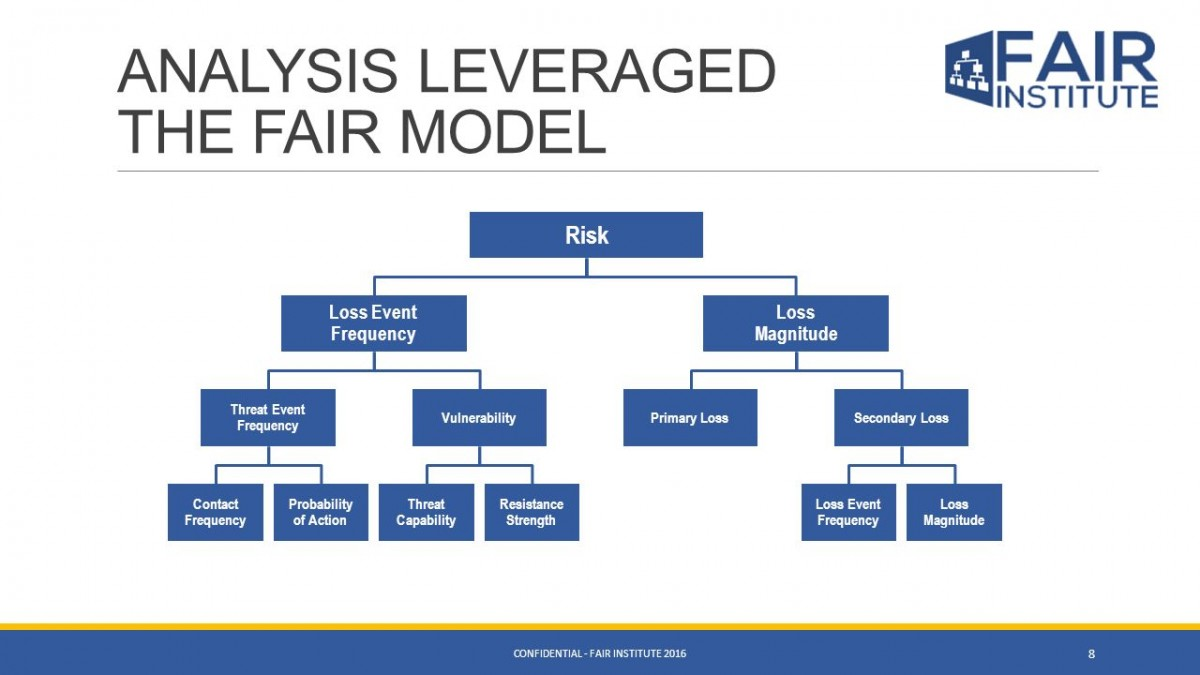
\includegraphics[width=0.8\textwidth]{img/FAIR-Cyber-Risk-Quantification-model.png}
    \caption{FAIR Siber Risk Nicelleştirme Modeli}
    \label{fig:fair-risk-model}
\end{figure}

FAIR metodolojisi, riski iki ana bileşene ayırır:
\begin{itemize}
    \item \textbf{Kayıp Olayı Frekansı (Loss Event Frequency - LEF):} Belirli bir süre zarfında bir kayıp olayının ne sıklıkta meydana gelme olasılığını ölçer.
    \item \textbf{Kayıp Büyüklüğü (Loss Magnitude - LM):} Bir kayıp olayının potansiyel etkisini finansal olarak ifade eder. Bu, birincil (üretkenlik kaybı, müdahale maliyeti) ve ikincil (itibar kaybı, yasal cezalar) kayıpları içerir.
\end{itemize}

\textbf{Pratik FAIR Analiz Senaryosu: Bir Çalışanın Dizüstü Bilgisayarının Çalınması}

\begin{itemize}
    \item \textbf{Senaryo:} "Ayrıcalıklı bir çalışanın, hassas müşteri verilerini içeren dizüstü bilgisayarının çalınmasıyla ilişkili riski analiz edin".
    \item \textbf{Adım 1: Değerleme (Varlık Değeri):} Varlığın değeri sadece fiziksel cihaz değil, asıl olarak içerdiği hassas veridir (PII, entelektüel mülkiyet, vb.).
    \item \textbf{Adım 2: Tek Kayıp Beklentisi (Single Loss Expectancy - SLE) Hesaplaması:} Bu, tek bir olaydan kaynaklanan maliyettir.
    \begin{itemize}
        \item \textbf{Formül:} SLE = Varlık Değeri $\times$ Maruz Kalma Faktörü
        \item \textbf{Örnek Uygulama:}
        \begin{itemize}
            \item Varlık Değeri: \$2.500 (laptop) + \$22.500 (hassas PII verisi, önceki olaylara göre belirlenen yasal maliyetler, itibar kaybı vb.) = \textbf{\$25.000}.
            \item Maruz Kalma Faktörü: Şifrelenmemiş veriye sahip bir laptop çalındığında bu \%100'dür.
            \item SLE: \$25.000 $\times$ \%100 = \$25.000
        \end{itemize}
    \end{itemize}
    \item \textbf{Adım 3: Yıllık Meydana Gelme Oranı (Annual Rate of Occurrence - ARO) Hesaplaması:} Bu, yılda kaç kez bu tür bir olayın meydana gelmesinin beklendiğidir.
    \begin{itemize}
        \item \textbf{Örnek Uygulama:} Geçmiş olaylara bakılarak, yılda ortalama 11 laptop hırsızlığı yaşanmışsa, ARO değeri \textbf{11}'dir.
    \end{itemize}
    \item \textbf{Adım 4: Yıllık Kayıp Beklentisi (Annual Loss Expectancy - ALE) Hesaplaması:} Bu, bir riskten kaynaklanan yıllık maliyet beklentisidir.
    \begin{itemize}
        \item \textbf{Formül:} ALE = SLE $\times$ ARO
        \item \textbf{Örnek Uygulama:} \$25.000 $\times$ 11 = \$275.000
    \end{itemize}
\end{itemize}

Aşağıdaki tablo, bu FAIR analiz senaryosunu özetlemektedir:

\begin{center}
\begin{tabularx}{0.95\textwidth}{|>{\raggedright\arraybackslash}X|>{\raggedright\arraybackslash}X|>{\centering\arraybackslash}X|}
\hline
\textbf{Bileşen} & \textbf{Tanım} & \textbf{Değer} \\
\hline
\textbf{Varlık} & Çalınan dizüstü bilgisayarın değeri, içerdiği hassas PII verisi dahil & 25.000\$ \\
\hline
\textbf{Tek Kayıp Beklentisi (SLE)} & Tek bir olayın maliyeti (\$25.000 $\times$ \%100 maruz kalma faktörü) & 25.000\$ \\
\hline
\textbf{Yıllık Meydana Gelme Oranı (ARO)} & Yılda beklenen olay sayısı & 11 \\
\hline
\textbf{Yıllık Kayıp Beklentisi (ALE)} & Yıllık toplam beklenen maliyet (\$25.000 $\times$ 11) & 275.000\$ \\
\hline
\end{tabularx}
\end{center}

Bu tür nicel veriler, soyut bir tehdidi finansal terimlere dökerek, güvenlik yöneticilerinin üst yönetimle aynı dilde konuşmasını sağlar ve bütçe gerekçelendirmesini kolaylaştırır.

\subsection{Risk Appetite ve Tolerance Definition (Risk İştahı ve Tolerans Tanımı)}

Risk iştahı, organizasyonun hedeflerini takip ederken kabul etmeye istekli olduğu genel risk seviyesidir. Risk toleransı ise, belirli bir risk türü için kabul edilebilir varyasyonun daha granüler bir yansımasıdır. Risk toleransı, risk iştahı doğrultusunda, belirli sınırlar ve eşikler belirler.

\subsection{Risk Treatment Strategies ve Control Selection (Risk Ele Alma Stratejileri ve Kontrol Seçimi)}

Risk değerlendirmesi tamamlandıktan sonra, kuruluşlar riskleri yönetmek için stratejiler belirler. Başlıca stratejiler şunlardır:
\begin{itemize}
    \item \textbf{Kaçınma (Avoidance):} Riski tamamen ortadan kaldırmak için ilgili aktiviteyi veya sistemi terk etme. Örneğin, hassas verileri güvensiz bir bulut hizmetinde depolamaktan kaçınmak.
    \item \textbf{Azaltma (Loss Prevention and Reduction):} Kontroller uygulayarak bir olayın oluşma sıklığını veya etkisini azaltma. Bu, en yaygın siber güvenlik stratejisidir. Örneğin, güvenlik duvarları ve şifreleme kullanmak.
    \item \textbf{Transfer Etme (Transfer):} Riski finansal olarak başka bir tarafa devretme. En yaygın örneği siber sigorta almaktır. Bu, riskin finansal yükünü sigorta şirketine aktarır.
    \item \textbf{Kabul Etme (Retention):} Riski bilerek ve isteyerek kabul etme ve sonuçlarına katlanma kararı. Bu, riski yönetmenin maliyetinin, riskin gerçekleşme olasılığı veya etkisinden daha yüksek olduğu durumlarda tercih edilebilir.
\end{itemize}

\subsection{OCTAVE FORTE Risk Değerlendirme Metodolojisi}



OCTAVE FORTE (Operationally Critical Threat, Asset, and Vulnerability Evaluation), Carnegie Mellon Üniversitesi tarafından geliştirilen sistematik bir bilgi güvenliği risk değerlendirme metodolojisidir. Bu çerçeve, organizasyonların kritik varlıklarını belirlemelerine, tehditleri değerlendirmelerine ve risk azaltma stratejileri geliştirmelerine yardımcı olur.

\section{Uyum Yönetimi ve Düzenleyici Çerçeveler}

Uyum (compliance), bir organizasyonun yasalara, düzenlemelere ve standartlara uyma eylemidir. Yönetişim içsel hedeflerle ilgiliyken, uyumluluk dışsal gereksinimlere odaklanır.

\subsection{Regulatory Compliance Assessment ve Gap Analysis (Düzenleyici Uyum Değerlendirmesi ve Açık Analizi)}

Açık analizi (gap analysis), bir kuruluşun mevcut politika, prosedür ve uygulamalarını belirli bir düzenleyici çerçeveye (örneğin, GDPR, HIPAA) göre değerlendirerek eksiklikleri belirleme sürecidir.

\textbf{Adım Adım Gap Analizi:}
\begin{enumerate}
    \item \textbf{Kapsamı Tanımlayın:} Hangi düzenlemelere ve standartlara uyum sağlanması gerektiğini net bir şekilde belirleyin.
    \item \textbf{Mevcut Durumu Gözden Geçirin:} Mevcut politikaları, kontrolleri ve prosedürleri kapsamlı bir şekilde inceleyin. Bu, belgeleme, uygulamalar ve teknolojileri içerir.
    \item \textbf{Açıkları Belirleyin:} Mevcut durum ile uyum gereklilikleri arasındaki tutarsızlıkları listeleyin. Bu, eksik kontrolleri, güncel olmayan politikaları veya eksik belgeleri içerebilir.
    \item \textbf{Açıkları Önceliklendirin:} Her açığı, potansiyel etkisi ve risk seviyesine göre sıralayın. Örneğin, müşteri verilerinin şifrelenmemesi, ağır finansal cezalara ve itibar kaybına yol açabileceği için yüksek öncelikli bir açık olabilir.
\end{enumerate}

\subsection{Internal Audit Programs ve Control Testing (Kurum İçi Denetim Programları ve Kontrol Testi)}

Kurum içi denetim programları, siber güvenlik süreçlerinin, politikalarının ve araçlarının etkinliğini değerlendirmek ve potansiyel tehditlere karşı uygun kontrollerin mevcut olduğunu doğrulamak için kritik öneme sahiptir. Bu denetimler, riskleri belirlemeye ve gidermeye yardımcı olurken, aynı zamanda dış denetimlere hazırlık sağlar.

\subsection{External Audit Coordination ve Remediation Management (Dış Denetim Koordinasyonu ve İyileştirme Yönetimi)}

Dış denetimler, üçüncü bir tarafın uyumluluğu doğrulaması için yapılır. Başarılı bir dış denetim, titiz bir hazırlık ve denetim bulgularının etkin bir şekilde giderilmesini gerektirir. Uyum otomasyon araçları, denetim sürecini kolaylaştırarak kanıt toplama ve raporlama yükünü azaltır.

\subsection{Compliance Automation Tools ve Continuous Monitoring (Uyum Otomasyon Araçları ve Sürekli İzleme)}

Sürekli uyum, kuruluşun uyumluluk gerekliliklerini yıl boyunca sürekli olarak izlemesini ve uyumsuzluk sorunlarını ortaya çıktıkça gerçek zamanlı olarak gidermesini sağlayan bir süreçtir. Bu, uyumu tek bir yıllık denetim etkinliğinden sürekli bir sürece dönüştürür.

Bu otomasyon, geleneksel manuel süreçlerin zaman alıcı ve kaynak yoğun doğasını ortadan kaldırır. Otomasyon araçları (SIEM, SOAR), kanıt toplama ve kontrol testini otomatikleştirerek insan müdahalesini \%80 oranında azaltabilir. Bu, kuruluşların denetime hazır olma süresini haftalara indirebilir ve proaktif bir duruşa geçişi temsil eder.

\textbf{Sürekli İzleme İçin Temel Araçlar:}
\begin{itemize}
    \item \textbf{Güvenlik Bilgileri ve Olay Yönetimi (SIEM):} SIEM araçları (Splunk, IBM QRadar, SolarWinds Security Event Manager) çeşitli kaynaklardan (sunucular, uygulamalar, ağ cihazları) gelen logları ve olay verilerini toplar, normalleştirir ve ilişkilendirir. Bu, gerçek zamanlı olarak tehditleri ve güvenlik ihlallerini tespit etmeyi sağlar. Örneğin, bir sağlık kuruluşu, HIPAA uyumluluğunu sağlamak için bir SIEM kullanır. SIEM, elektronik sağlık kayıtlarına yetkisiz erişimi izler ve raporlar oluşturur.
    \item \textbf{Siber Güvenlik Orkestrasyonu, Otomasyonu ve Müdahalesi (SOAR):} SOAR platformları, SIEM'den gelen uyarıları alır ve önceden tanımlanmış "playbook"lar (oyun planları) aracılığıyla otomatik veya yarı otomatik müdahale eylemleri başlatır.
\end{itemize}

\textbf{Örnek SOAR Playbook (Oltalama Saldırısı Müdahalesi):}
\begin{enumerate}
    \item \textbf{Algılama:} SIEM, bir e-posta güvenliği ağ geçidinden şüpheli bir e-posta uyarısı alır.
    \item \textbf{Sınıflandırma ve Analiz:} SOAR, e-postadaki göstergeleri (URL, IP, dosya hash'leri) otomatik olarak çıkarır ve üçüncü taraf tehdit istihbaratı araçlarıyla karşılaştırır. Bu analiz, e-postanın kötü amaçlı olup olmadığını doğrular.
    \item \textbf{İçerme (Containment):} Eğer e-posta kötü amaçlı olarak doğrulanırsa, SOAR tüm kullanıcıların gelen kutularındaki şüpheli e-postaları otomatik olarak karantinaya alır ve ilgili etki alanlarını güvenlik duvarı seviyesinde engeller.
    \item \textbf{Kaldırma (Eradication):} Analiz tamamlandıktan sonra, SOAR tehdidin etkisiz hale getirildiğini doğrular ve ilgili güvenlik olayını kapatır.
\end{enumerate}

\subsection{Cross-border Compliance ve Data Sovereignty (Sınır Ötesi Uyum ve Veri Egemenliği)}

Veri egemenliği, dijital verilerin üretildiği ülkenin yasalarına ve yönetişim yapılarına tabi olduğu ilkesidir. Bu durum, özellikle çok uluslu şirketler için sınır ötesi veri transferlerini karmaşık bir hale getirir.

\textbf{Yeterlilik Kararları (Adequacy Decisions):} Avrupa Komisyonu tarafından verilen bir yeterlilik kararı, AB dışındaki bir ülkenin kişisel veriler için yeterli düzeyde koruma sağladığını resmen onaylar. Bir ülke "yeterlilik" statüsü kazandığında, kişisel veriler AB'den bu ülkeye ek koruyucu önlemler (örneğin, Standart Sözleşme Maddeleri - SCC'ler) olmaksızın serbestçe akabilir. Bu, veri transfer süreçlerini teknik ve operasyonel olarak basitleştirir.

Yeterlilik kararı olmadığında, kuruluşlar veri transferlerini sağlamak için "uygun güvenceler" (appropriate safeguards) kullanmak zorundadır. Bu güvenceler şunları içerir:
\begin{itemize}
    \item \textbf{Standart Sözleşme Maddeleri (SCC'ler):} Bunlar, veri koruma yetkilileri tarafından onaylanmış ve veri transferinde kullanılması gereken yasal metinlerdir. Bu maddeler, transferin teknik olarak nasıl gerçekleştirileceğini (şifreleme, erişim kontrolü vb.) dolaylı olarak etkileyebilir.
    \item \textbf{Bağlayıcı Şirket Kuralları (BCR'ler):} Çok uluslu şirketler için geçerli olan, dahili veri transferlerini yöneten, denetim makamları tarafından onaylanması gereken bağlayıcı kurallardır.
\end{itemize}

Bu durum, gizlilik mühendisliği kontrollerinin (örneğin, şifreleme) yalnızca iyi bir uygulama değil, aynı zamanda belirli yasal durumlarda zorunlu bir gereklilik haline geldiğini göstermektedir.

\section{Güvenlik Metrikleri, KPIs ve Performans Ölçümü}

Güvenlik metrikleri ve temel performans göstergeleri (KPI'lar), bir siber güvenlik programının etkinliğini ölçmek, tehdit eğilimlerini anlamak ve yatırım kararlarını gerekçelendirmek için kullanılır. Bu veriler, güvenlik durumunun tarihsel bir perspektifini sunarak, zaman içindeki eğilimleri ve değişiklikleri görmeyi sağlar.

\subsection{Security Performance Indicator Development (Güvenlik Performans Göstergesi Geliştirme)}

Güvenlik metrikleri, yatırımları izlemenin ötesine geçerek tehdit modelleri, olay müdahale verimliliği ve sistem zafiyetleri hakkında içgörüler sunar. Bu göstergeler, güvenlik stratejilerinin ne kadar etkili olduğunu anlamak için kritik öneme sahiptir.
\begin{itemize}
    \item \textbf{KPI Örnekleri:}
    \begin{itemize}
        \item Algılama Süresi (Mean Time to Detect - MTTD) ve Müdahale Süresi (Mean Time to Respond - MTTR).
        \item Yamalı ve güncel cihazların yüzdesi.
        \item Siber güvenlik farkındalık eğitimi tamamlama oranı.
        \item Saldırı girişimlerinin sayısı.
    \end{itemize}
\end{itemize}

\subsection{Risk Metrics ve Trend Analysis (Risk Metrikleri ve Trend Analizi)}

Risk metrikleri, riskin parasal terimlerle nicelleştirilmesine olanak tanır ve zaman içindeki eğilimleri analiz etmeye yardımcı olur. Bir statik sayıdan ziyade, zaman içindeki ilerlemeyi gösteren bir trend çizgisi, üst yönetim için daha anlamlıdır.
\begin{itemize}
    \item \textbf{Kullanım Alanları:}
    \begin{itemize}
        \item \textbf{Nicel Risk Değerleri:} FAIR metodolojisinden elde edilen Yıllık Kayıp Beklentisi (ALE) gibi metrikler, riski objektif olarak değerlendirmeyi sağlar.
        \item \textbf{Trend Analizi:} Güvenlik olaylarının sayısı veya bir riskin parasal değeri, düzenli aralıklarla izlenerek bir trend grafiği oluşturulabilir.
    \end{itemize}
\end{itemize}

\subsection{Executive Dashboard Design ve Reporting (Yönetici Kontrol Paneli Tasarımı ve Raporlama)}

Yöneticilere yönelik bir kontrol paneli, kapsamlı ve teknik verilerde kaybolmadan yüksek seviyeli risk, uyumluluk ve stratejik hedeflere doğru ilerleme hakkında genel bir bakış sunar.

\textbf{Tasarım İlkeleri:}
\begin{enumerate}
    \item \textbf{Hedef Kitleyi Tanıyın:} Yönetim kurulu üyeleri stratejik kararlar alırlar, bu nedenle raporlar finansal etki, risk azaltma ve iş değeri gibi konulara odaklanmalıdır.
    \item \textbf{Sadelik:} Dashboard, beş ila altı temel "kart" veya bileşenle sınırlı olmalı ve trafik ışığı protokolü (kırmızı, sarı, yeşil) gibi basit görsel ipuçları kullanmalıdır.
    \item \textbf{Hikaye Anlatma:} Statik veriler yerine, zaman içindeki ilerlemeyi gösteren trend çizgileri kullanılmalıdır. Bu, güvenlik yatırımlarının işe yaradığını gösteren bir hikaye anlatmaya yardımcı olur.
\end{enumerate}

\textbf{Örnek Dashboard Metrikleri:}
\begin{itemize}
    \item Genel Risk Skoru (Nicel bir değer)
    \item Politikalara Uyum Seviyesi (Yüksek, Orta, Düşük)
    \item MTTD ve MTTR Trendleri
    \item Saldırı Girişimleri Sayısı ve Kaynağı
\end{itemize}

\subsection{Security Investment ROI Calculation (Güvenlik Yatırımı ROI Hesaplaması)}

Güvenlik yatırımlarının geri dönüşünü (ROSI), geleneksel finansal ROI formüllerinin ötesinde, azaltılan potansiyel kayıplar üzerinden hesaplamak gerekir.

\begin{equation}
ROSI = \frac{(ALE \times \text{Azaltma Oranı}) - \text{Çözüm Maliyeti}}{\text{Çözüm Maliyeti}}
\end{equation}

\textbf{Örnek Senaryo:}
\begin{itemize}
    \item \textbf{Senaryo:} Fidye yazılımı ve DDoS saldırılarına karşı bir Yönetilen Güvenlik Hizmeti Sağlayıcısı (MSSP) çözümü almayı değerlendiren bir kuruluş.
    \item \textbf{Veriler:} Fidye yazılımı ve DDoS için beklenen toplam yıllık kayıp beklentisi (ALE) 41.500.000\$. Çözümün bu tehditleri önlemedeki etkinliği (azaltma oranı) \%80 ve yıllık maliyeti 120.000\$.
    \item \textbf{Hesaplama:}
    \begin{equation*}
    ROSI = \frac{(41,500,000 \times 0.8) - 120,000}{120,000} = 275.67 = 27,567\%
    \end{equation*}
\end{itemize}

Güvenlik yatırımları doğrudan gelir getirmediği için finans ekipleri için değeri genellikle belirsizdir. ROSI formülü, bu soyut yararı (azaltılan risk) somut, parasal bir değere dönüştürür. Yapılan hesaplama, her bir dolarlık güvenlik yatırımının 275 dolar potansiyel kaybı önlediğini gösterir. Bu nicel veri, yöneticilerin bütçe kararlarını gerekçelendirmesine yardımcı olur.

\subsection{Benchmark Analysis ve Peer Comparison (Kıyaslama Analizi ve Akran Karşılaştırması)}

Kıyaslama analizi, bir organizasyonun güvenlik duruşunu sektördeki veya benzer büyüklükteki akranlarına göre değerlendirme sürecidir. Bu, kuruluşun kendi performans hedeflerini belirlemesine ve yatırım yapılacak alanlara odaklanmasına yardımcı olur. Etkin kıyaslama için, yüksek kaliteli veri, ortak bir terminoloji ve karşılaştırılabilir metriklerin kullanımı esastır.

\section{İş Sürekliliği ve Felaket Kurtarma Planlaması}

İş sürekliliği planlaması (BCP), bir kriz anında temel iş süreçlerinin devamlılığını sağlamayı amaçlayan geniş kapsamlı bir yaklaşımdır. Felaket Kurtarma Planı (DRP) ise, BCP'nin teknolojiye odaklanan, veri kurtarma ve IT sistemlerini yeniden çalışır hale getirme üzerine yoğunlaşan bir alt kümesidir.

\subsection{Business Impact Analysis (BIA) ve Criticality Assessment (İş Etki Analizi ve Kritiklik Değerlendirmesi)}

BIA, bir olayın en önemli iş süreçlerini nasıl etkileyeceğini anlamak için kritik bir ilk adımdır. Bu analiz, varlıkların önceliklendirilmesine temel oluşturur ve kaynakların en kritik alanlara ayrılmasını sağlar. Adımlar, bir varlık envanteri oluşturmayı, varlıkları iş fonksiyonlarına göre kritikliklerine göre sıralamayı ve potansiyel etkilerini değerlendirmeyi içerir.

\subsection{Recovery Time Objective (RTO) ve Recovery Point Objective (RPO) (Kurtarma Süresi ve Kurtarma Noktası Hedefi)}

Bu hedefler, bir felaket durumunda kurtarmanın nasıl önceliklendirileceğini ve ne kadar hızlı gerçekleşeceğini belirler.
\begin{itemize}
    \item \textbf{RTO (Recovery Time Objective):} Bir uygulamanın, işi olumsuz etkilemeye başlamadan önce maksimum kapalı kalabileceği süredir.
    \item \textbf{RPO (Recovery Point Objective):} Bir kesinti anında kabul edilebilir maksimum veri kaybı miktarıdır. Bu, veri yedekleme sıklığını belirler.
\end{itemize}

Aşağıdaki tablo, farklı iş süreçleri için RTO ve RPO hedeflerini kritiklik seviyelerine göre sınıflandırmaktadır:

\begin{center}
\begin{longtable}{|>{\raggedright\arraybackslash}p{3cm}|>{\raggedright\arraybackslash}p{3cm}|>{\centering\arraybackslash}p{2.5cm}|>{\centering\arraybackslash}p{2.5cm}|}
\caption{İş Kritikliği Seviyelerine Göre RTO ve RPO Hedefleri} \\
\hline
\textbf{İş Kritikliği Seviyesi} & \textbf{Örnek İş Süreci} & \textbf{RTO (Kurtarma Süresi)} & \textbf{RPO (Kurtarma Noktası)} \\
\hline
\endfirsthead
\multicolumn{4}{l}{\small\tablename\ \thetable\ -- devamı} \\
\hline
\textbf{İş Kritikliği Seviyesi} & \textbf{Örnek İş Süreci} & \textbf{RTO (Kurtarma Süresi)} & \textbf{RPO (Kurtarma Noktası)} \\
\hline
\endhead
\hline
\multicolumn{4}{r}{\small Devamı sonraki sayfada} \\
\endfoot
\hline
\endlastfoot
\textbf{Görev-Kritik (Mission-Critical)} & Müşteri Sipariş Sistemi, Finansal İşlemler & Saniyelerden Dakikalara & 0-15 dakika \\
\hline
\textbf{Temel (Essential)} & E-posta, İK Uygulamaları & 4 ila 24 saat & 1-24 saat \\
\hline
\textbf{Kritik Olmayan (Nonessential)} & İç Raporlama Araçları, İdari Dosyalama & 24 saatten Haftalara & 24 saatten haftalara \\
\end{longtable}
\end{center}

Bu matris, IT ve iş ekiplerinin kurtarma öncelikleri üzerinde ortak bir anlayışa sahip olmasını sağlar, böylece kaynaklar en acil ihtiyaçlara yönlendirilebilir.

\subsection{Disaster Recovery Planning ve Testing (Felaket Kurtarma Planlaması ve Testi)}

DRP, siber saldırı, doğal afet veya sistem arızası gibi olaylara müdahale etmek için stratejiler ve protokoller sağlayan bir yol haritasıdır. Bir DRP'nin var olması yeterli değildir; planın gerçek bir kriz anında işe yaradığından emin olmak için düzenli olarak test edilmesi ve güncellenmesi gerekir.

\textbf{Plan Oluşturma Adımları:}
\begin{enumerate}
    \item \textbf{Ekip Kurma:} Kriz anında müdahale çabalarına liderlik edecek bir afet müdahale ekibi oluşturun.
    \item \textbf{Altyapı Planı:} Ağ altyapınızın ve sistem bağımlılıklarının detaylı bir planını çizin.
    \item \textbf{Kurtarma Prosedürlerini Belgeleyin:} Hasarlı sistemleri, uygulamaları ve verileri kurtarmak için adım adım talimatları basit bir dille yazın. Bu plan ağdan uzak bir yerde veya değişmez (immutable) depolama alanında saklanmalıdır.
\end{enumerate}

\textbf{Test ve Tatbikat Türleri:}
\begin{itemize}
    \item \textbf{Masaüstü Tatbikatları (Tabletop Exercises):} Ekip, bir senaryoyu (örneğin, fidye yazılımı saldırısı) sözlü olarak tartışır, rolleri ve prosedürleri gözden geçirir.
    \item \textbf{Simülasyonlar:} Gerçek bir kesintiyi simüle ederek, sistemlerin kurtarma kabiliyetini test eder. Bu testler, planın zayıf yönlerini ortaya çıkarır ve bu eksiklikler, gerçek bir olaydan önce giderilebilir.
\end{itemize}

\subsection{Crisis Management ve Emergency Response (Kriz Yönetimi ve Acil Durum Müdahale)}

Bir siber saldırı, özellikle fidye yazılımı (ransomware), özel bir müdahale planı gerektirir. Aktörlerin sizi izleyebileceği düşünülerek, müdahale işlemleri koordineli bir şekilde ve bant dışı (out-of-band) iletişim kanalları (telefon görüşmeleri) kullanılarak yapılmalıdır.

\textbf{Fidye Yazılımı Müdahale ve Kurtarma Planı (Teknik Playbook):}
\begin{enumerate}
    \item \textbf{İçerme (Containment):} Ağdaki enfekte sistemleri hemen belirleyin ve yalıtın.
    \begin{itemize}
        \item \textbf{Teknik Adımlar:} Etkilenen sistemlerin ağ kablosunu çekin veya kablosuz bağlantısını kesin. Enfeksiyonun yayılmasını engellemek için anahtar (switch) seviyesinde ağı kapatmak en etkili yöntem olabilir.
    \end{itemize}
    \item \textbf{Delil Toplama:} Forensik inceleme için etkilenen sistemlerin imajını alın ve uçucu hafıza içeriğini (volatile memory) yakalayın.
    \item \textbf{Temizleme (Eradication):} Tüm enfekte sistemleri silin veya dezenfekte edin.
    \item \textbf{Kurtarma ve Yeniden İnşa:} Yedeklerden geri yüklemeye başlayın.
\end{enumerate}

\begin{verbatim}
--Veritabanı Geri Yükleme (SQL Server Örneği):
RESTORE DATABASE [veritabani_adi] \
    FROM DISK = '[yedek_dosyasi_yolu]' \
    WITH RECOVERY
\end{verbatim}

\begin{verbatim}
--Anlık Görüntü (Snapshot) Geri Yükleme (AWS RDS Örneği):
aws rds restore-db-cluster-from-snapshot \
    --db-cluster-identifier my-db-cluster \
    --snapshot-identifier my-snapshot-id \
    --engine aurora-postgresql
\end{verbatim}

\begin{verbatim}
--Dosya Geri Yükleme (Linux Örneği):
restore -xvqf /dev/rmt0 /home/mike/tools
\end{verbatim}

\subsection{Supply Chain Continuity ve Vendor Dependency Management (Tedarik Zinciri Sürekliliği ve Tedarikçi Bağımlılık Yönetimi)}

İşletmelerin giderek daha karmaşık hale gelen tedarik zincirlerine bağımlı olması, bu zincirdeki kesintilere karşı dayanıklılık oluşturmayı zorunlu hale getirir. Bu dayanıklılığı artırmak için şu stratejiler benimsenmelidir:
\begin{itemize}
    \item \textbf{Proaktif Tanımlama:} Kritik vendor bağımlılıklarını önceden belirleyin ve tek kaynaklı tedarik anlaşmalarının potansiyel tehlikelerini anlayın.
    \item \textbf{Alternatif Kaynak Geliştirme:} Kriz anında hızlı geçişi mümkün kılmak için önceden nitelikli, alternatif tedarikçilerle ilişkiler kurun.
    \item \textbf{SLA ve Sözleşme Güçlendirme:} Kesinti anında tedarikçi sorumluluklarını netleştiren güçlü sözleşmeler hazırlayın.
\end{itemize}

\section{Gizlilik Yönetimi ve Veri Koruma Yönetişimi}

Gizlilik yönetimi, özellikle kişisel verilerin korunmasına odaklanan GRC'nin kritik bir bileşenidir.

\subsection{Privacy by Design ve Privacy Impact Assessments (Tasarım Yoluyla Gizlilik ve Gizlilik Etki Değerlendirmeleri)}

Tasarım yoluyla gizlilik (Privacy by Design), gizliliği bir sistemin veya projenin başlangıç tasarımından itibaren entegre etme ilkesidir. Gizlilik Etki Değerlendirmesi (PIA), bu ilkenin pratik bir uygulamasıdır. PIA, özellikle kişisel verilerin işlenmesi yüksek risk taşıyorsa veya yeni teknolojiler kullanılıyorsa zorunludur.

\subsection{Data Protection Officer (DPO) Role ve Responsibilities (Veri Koruma Görevlisi Rolü ve Sorumlulukları)}

Veri Koruma Görevlisi (DPO), kuruluşun veri koruma kurallarına uyumunu sağlamaktan sorumlu kilit bir pozisyondur.
\begin{itemize}
    \item \textbf{Temel Sorumlulukları:} Yönetime ve çalışanlara veri koruma yükümlülükleri hakkında danışmanlık yapmak, uyumluluğu izlemek ve veri sahiplerinden gelen talepler için iletişim noktası olmak.
    \item \textbf{DPO'nun Konumu:} DPO, görevlerini bağımsız bir şekilde yerine getirebilmeli ve yönetim çatışmasından kaçınmak için diğer görevlerle çelişmemelidir.
\end{itemize}

\subsection{Data Subject Rights Management ve Breach Notification (Veri Sahibi Hakları Yönetimi ve İhlal Bildirimi)}

Veri sahipleri, kişisel verileri üzerinde belirli haklara sahiptir. Kuruluşlar, bu hakları yönetmek için süreçler kurmalıdır. Kişisel veri ihlali durumunda, kontrolör, mümkünse ihlalin farkına vardıktan sonra en geç 72 saat içinde yetkili denetim makamına bildirimde bulunmalıdır. Eğer ihlal veri sahipleri için yüksek risk oluşturuyorsa, doğrudan bildirim zorunludur.

\subsection{Cross-border Data Transfer ve Adequacy Decisions (Sınır Ötesi Veri Transferi ve Yeterlilik Kararları)}

Bir yeterlilik kararı, veri egemenliği sorunlarını azaltarak teknik akışı kolaylaştıran bir yasal mekanizma sağlar. Yeterlilik kararı, veri transferi mekanizmaları üzerindeki teknik yükü doğrudan etkiler. Bu karar olmadığında, kuruluşlar daha karmaşık mekanizmalar kullanmak zorundadır. Bu, Standart Sözleşme Maddeleri (SCC'ler) veya Bağlayıcı Şirket Kuralları (BCR'ler) gibi "uygun güvenceler"in kullanılmasını gerektirir. Bu durum, gizlilik mühendisliği kontrollerinin (örneğin, şifreleme) sadece iyi bir uygulama değil, aynı zamanda belirli yasal durumlarda zorunlu bir gereklilik haline geldiğini gösterir.

\subsection{Privacy Engineering ve Technical Controls Implementation (Gizlilik Mühendisliği ve Teknik Kontroller Uygulaması)}

Gizlilik mühendisliği, kişisel verileri işleyen sistemlerin ve hizmetlerin tasarımına gizlilik ilkelerini dahil eden bir disiplindir. Bu, veri anonimleştirme ve şifreleme gibi teknikleri içerir.

\textbf{Veri Anonimleştirme ve Gizlilik Koruma Teknikleri:}
\begin{itemize}
    \item \textbf{K-Anonimlik:} Bir veri setinde, her bir birey için en az k-1 diğer bireyin verileriyle ayırt edilemez olmasını sağlayan bir özelliktir. Örneğin, bir hastane veritabanında, yaş ve cinsiyet gibi yarı tanımlayıcı (quasi-identifier) veriler genelleştirilerek (örneğin, 20-30 yaş arası erkek), saldırganın bir bireyi diğerlerinden ayırt etmesi engellenir. Bu tekniğin, saldırganın arka plan bilgisi varsa başarısız olabileceği bir sınırlılığı bulunmaktadır.
    \item \textbf{Diferansiyel Gizlilik (Differential Privacy):} Bir veri setine istatistiksel sorgular yapılırken, bireysel bir kaydın varlığının veya yokluğunun sorgu sonucunu önemli ölçüde etkilemesini önlemek için dikkatli bir şekilde gürültü (noise) ekleme tekniğidir. Bu teknik, özellikle büyük veri setlerinin analizi sırasında her bir bireyin gizliliğini korumak için kullanılır.
\end{itemize}

\textbf{Veri Anonimleştirme ve Maskeleme Teknikleri:}

\begin{itemize}
    \item \textbf{Maskeleme}
    \begin{itemize}
        \item \textbf{Tanım:} Gerçek verilerin yerine farklı, ancak kullanışlı veriler koyma
        \item \textbf{Uygulama Örneği:} Bir veritabanındaki müşteri adının J*** S**** şeklinde değiştirilmesi
    \end{itemize}
    
    \item \textbf{Anonimleştirme}
    \begin{itemize}
        \item \textbf{Tanım:} Verileri, başka verilerle eşleştirilerek dahi hiçbir şekilde belirli bir kişiyle ilişkilendirilemeyecek hale getirme
        \item \textbf{Uygulama Örneği:} Çalışan yaşlarının tek tek gösterilmesi yerine, "X yaşında Z kadar çalışan var" şeklinde genelleştirilmesi
    \end{itemize}
    
    \item \textbf{K-Anonimlik}
    \begin{itemize}
        \item \textbf{Tanım:} Bir veri setindeki her bir kaydın, en az k diğer kayıtla ayırt edilemez olmasını sağlama
        \item \textbf{Uygulama Örneği:} 19 yaşında bir hastanın yaşının "20 ve altı" olarak genelleştirilmesi
    \end{itemize}
    
    \item \textbf{Pseudonymization}
    \begin{itemize}
        \item \textbf{Tanım:} Özel tanımlayıcıların yerine takma adlar veya sahte tanımlayıcılar kullanma
        \item \textbf{Uygulama Örneği:} "Fred Jones" adının "John Q. Public" ile değiştirilmesi
    \end{itemize}
    
    \item \textbf{Hashing}
    \begin{itemize}
        \item \textbf{Tanım:} Veriyi tek yönlü bir algoritmaya dönüştürerek orijinal veriye geri dönülmesini engelleme
        \item \textbf{Uygulama Örneği:} Bir IP adresinin statik bir tuz (salt) ile birleştirilerek hash'lenmesi
    \end{itemize}
\end{itemize}
